\chapter{Background}
\label{chap:background}

\setcounter{minitocdepth}{1}
\justifying
\textit{
This chapter presents the background on test flakiness, machine learning and spectrum-based fault localisation, essential for a good understanding of the different technical aspects of this dissertation. 
}


\chapterPage{
}

\section{Test Flakiness: Definition, Characteristics and Examples}


\subsection{Definition}
In English, we refer as \textit{flaky}, a person that is unreliable or someone that is behaving in a way that is strange, not responsible or not expected. This explains the origin of the appellation flaky test. While generally used by developers and practitioners to characterize tests that intermittently fail for no apparent reason, a general definition for a flaky test is commonly adopted by the research community: \\ 

\textbf{A flaky test is a test that passes and fails when executed multiple times on the same code.} \\

% Add flake rate

\subsection{Examples}

\begin{figure}[ht]
\centering
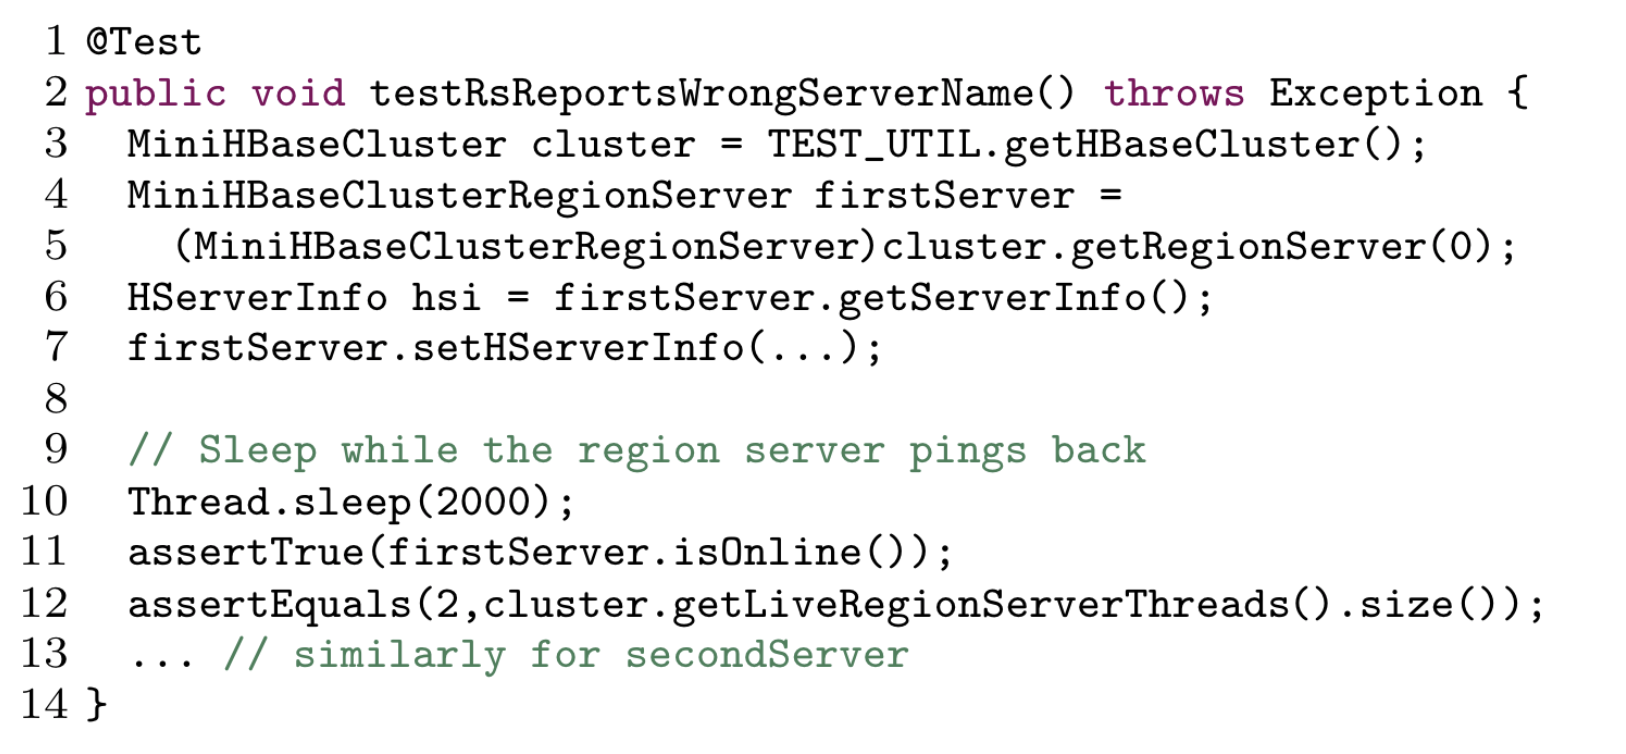
\includegraphics[width=1\textwidth]{figures/core/exampleAsync.png}
\caption{Example of a flaky test caused by an asynchronous wait~\cite{Luo2014}}
\label{fig:exampleAsync}
\end{figure}

Figure~\ref{fig:exampleAsync} shows a unit test written in Java for the HBase project. This test is flaky and was reported by Luo \etal in their empirical study. We can see that the test uses a \textsc{cluster} to initiate the server \textsc{firstServer}. Then, it waits for the server to ping back by using an asynchronous wait with \textsc{Thread.sleep(2000)}. We know that this test was sometimes passing and sometimes failing depending on how fast the server was put online.


\begin{figure}[ht]
\centering
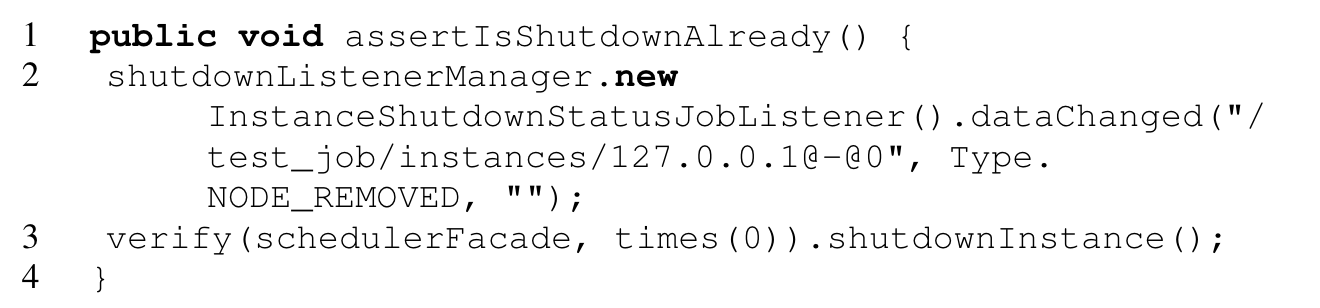
\includegraphics[width=1\textwidth]{figures/core/exampleOD.png}
\caption{Example of an order-dependent flaky test caused~\cite{Lam2019iDFlakies}}
\label{fig:exampleOD}
\end{figure}

Figure~\ref{fig:exampleOD} shows another flaky test taken in Elastic-Job, another popular Java project on GitHub. This test does not initially appear to be flaky, however, it was found by the iDFlakies tool as an order-dependent test. In their paper, Lam \etal explain that this test is checking that an instance of a class variable is shut down on line 3. It happens that this instance is started by another test and thus, depending on the order of executions in the test suite, this test can pass or fail. 


\subsection{Categories}
Several studies were conducted in an attempt to categorise flaky tests based on their root causes~\cite{parry2022surveying,Luo2014,Gruber2021,Lam2020a,Eck2019}. The categories slightly differ depending on the programming languages but the prevalent ones remain. Table~\ref{table:flakyniessCategories} list the most common flakiness categories.

% Table: Flakiness categories
\begin{table}[ht]
%\vspace{1.0em}
\centering
\caption{The different categories of flakiness commonly reported by the literature.}
\label{table:flakyniessCategories}

\resizebox{\textwidth}{!}{\begin{tabular}{c|p{10cm}|c}
\toprule
\textbf{Category} & \textbf{Definition} & \textbf{Sources} \\
\midrule
\multirow{4}{*}{Asynchronous Waits} & Flakiness caused by tests that involve asynchronous operations and have dependencies on timing, resulting in inconsistent behaviour if the expected response is not received within a specified time. & \multirow{4}{*}{~\cite{Eck2019,Gruber2021,Luo2014,Lam2020a}}\\
\midrule
\multirow{4}{*}{Concurrency} & Flakiness caused by race conditions or synchronization issues when multiple threads or processes interact with shared resources simultaneously, leading to unpredictable outcomes. & \multirow{4}{*}{~\cite{Eck2019,Gruber2021,Luo2014,Lam2020a}}\\
\midrule
\multirow{3}{*}{Time} & Tests depending on specific timing conditions, such as time-sensitive calculations or time-based events, and may produce different results based on the time of execution. & \multirow{3}{*}{~\cite{Eck2019,Gruber2021,Luo2014,Lam2020a}}\\
\midrule
\multirow{3}{*}{Order-Dependency} & Flakiness resulting from tests that rely on a specific execution order due to shared resources or dependencies, and may fail if the order among the tests is changed. & \multirow{3}{*}{~\cite{Eck2019,Gruber2021,Luo2014,Lam2020a}}\\
\midrule
\multirow{3}{*}{Randomness} & Flakiness caused by tests that involve random or pseudo-random behaviour, where different outcomes may occur on each run, potentially leading to inconsistent results. & \multirow{3}{*}{~\cite{Eck2019,Gruber2021,Luo2014,Lam2020a}}\\
\midrule
\multirow{3}{*}{Unordered Collections} & Flakiness resulting from tests that rely on unordered collections or sets, where the order of elements can vary, causing failures if the expected order is not maintained. & \multirow{3}{*}{~\cite{Gruber2021,Luo2014,Lam2020a}}\\
\hline
\multirow{4}{*}{Network} & Flakiness caused by network-related issues, such as unreliable connections, timeouts, or network congestion, leading to inconsistent results in tests that interact with remote services. & \multirow{4}{*}{~\cite{Eck2019,Gruber2021,Luo2014,Lam2020a}}\\
\midrule
\multirow{3}{*}{I/O (Input/Output)} & Flakiness resulting from tests that involve reading from or writing to external files, databases, or other I/O operations, where inconsistencies or errors can occur. & \multirow{3}{*}{~\cite{Eck2019,Gruber2021,Luo2014,Lam2020a}}\\
\midrule
\multirow{3}{*}{Resource Leak} & Flakiness caused by tests that do not release system resources properly, resulting in resource exhaustion and inconsistent behaviour when run repeatedly. & \multirow{3}{*}{~\cite{Eck2019,Gruber2021,Luo2014,Lam2020a}}\\
\midrule
\multirow{4}{*}{Floating Point} & Flakiness caused by tests that rely on the results of floating point operations, which can suffer from discrepancies and inaccuracies due to precision limitations, overflows, non-associative addition, and other factors. & \multirow{4}{*}{~\cite{Eck2019,Luo2014,Lam2020a}}\\
\midrule
\multirow{6}{*}{Platform Dependency} & Flakiness stemming from tests relying on specific functionalities of an operating system, library version, or hardware vendor. These dependencies can result in inconsistent and non-deterministic test failures, especially in cloud-based continuous integration environments where tests are executed on different platforms. & \multirow{6}{*}{~\cite{Gruber2021,Eck2019}}\\
\midrule
\multirow{3}{*}{Test Case Timeout} & Flakiness caused by tests that specify an upper limit for the test execution duration. Often those tests will fail because the instructions will not complete in time. & \multirow{3}{*}{~\cite{Eck2019,Gruber2021}}\\
\bottomrule
\end{tabular}}
\end{table}

% \paragraph{\textbf{Flake Rate}}


\section{Machine Learning}

Machine learning is a subfield of artificial intelligence focusing on the development of algorithms and models being able to learn and make predictions without being explicitly programmed. It involves the utilization of statistical techniques and computational power to analyze and interpret large datasets, identifying patterns and relationships within the data. By iteratively learning from many examples and experiences, machine learning algorithms improve their performance and can generalize to make accurate predictions or take informed actions on new, unseen data~\cite{mitchell2007machine,janiesch2021machine}. Machine learning can be divided into two subgroups: supervised learning and unsupervised learning.

\subsection{Supervised Learning}

Supervised learning is a machine learning approach relying on using labelled datasets. These datasets are collected and then used to train models, \ie supervising them, to classify data or to predict outcomes accurately. Supervised learning problems can further be divided into two families:

\begin{itemize}
    \item \textbf{Classification} problems aim at predicting the particular group or category for a data item. Famous examples of this problem are the binary classification of emails (spam or non-spam), or multi-class classification of a given handwritten character (one class for each letter in the alphabet). Common algorithms used for classification tasks include logistic regressions, support vector machines, decision trees and random forests.

    \item \textbf{Regression} problems aim at predicting a continuous numerical output variable based on input features. It involves building a regression model that can learn the relationship between the input variables (also known as independent variables, features, or predictors) and the output variable (also known as the dependent variable or target). Such an approach can be used to predict the price of houses based on features like living area and year of construction for example. Common algorithms used for regression tasks include linear regression, polynomial regression, decision tree regression, random forest regression, support vector regression, and neural network regression 
\end{itemize}


\subsection{Unsupervised Learning}

Unsupervised learning is a machine learning approach that learns to discover inherent patterns or relationships in the data and extract meaningful insights or representations without the need for labelled datasets. Unsupervised learning can also be subdivided into two groups:

\begin{itemize}
    \item \textbf{Clusering} algorithms group similar data points together based on their features or characteristics. The algorithm recognises patterns in the data and assigns data points to different clusters. Examples of clustering algorithms include k-means clustering, hierarchical clustering, or DBSCAN (Density-Based Spatial Clustering of Applications with Noise)~\cite{schubert2017dbscan,hartigan1979k}.

    \item \textbf{Dimension reduction} algorithms aim to reduce the number of features in a dataset while preserving important information. These algorithms transform high-dimensional data into a lower-dimensional representation. Principal Component Analysis (PCA) and t-SNE (t-Distributed Stochastic Neighbor Embedding) are commonly used dimensionality reduction techniques~\cite{van2008visualizing,abdi2010principal}.
\end{itemize}


\subsection{Performance Evaluation}
% Precision, Recall, F1, MCC, confusion matrix
Several chapters in this dissertation leverage supervised learning with binary or multi-class classification problems. To evaluate the performance of binary classification models, we rely on different metrics derived from true positives (TP), true negatives (TN), false positives (FP) and false negatives (FN). Precision measures the accuracy of positive predictions, while recall measures the completeness of positive predictions. In other words, precision measures how many detected items are relevant. It is calculated by dividing the true positives by the overall positive elements. Recall measures how many relevant elements were detected. Therefore it is calculated by dividing true positives by the number of relevant elements. 

    \[
    \textbf{Precision} = \frac{TP}{TP+FP} \quad \quad \quad \textbf{Recall} = \frac{TP}{TP+FN}
    \]

In addition to Precision and Recall, the F-score or F1 score is also often given. It's an accuracy measure calculated as the harmonic mean between Precision and Recall.

    \[
    \textbf{F1} = 2 \times \frac{Precision \times Recall}{Precision + Recall}
    \]
    
The accuracy of a model is sensitive to class imbalance. In particular, the precision and recall metrics can easily be impacted when one class is underrepresented. To alleviate this issue, we report the Matthews Correlation Coefficient (MCC) which is a more reliable statistical rate to avoid over-optimistic results in the case of an imbalanced dataset \cite{chicco2020advantages}.
This metric takes into consideration all four entries of the confusion matrix. MCC ranges from -1 to 1 and is given by the following formula: 
    \[
    \textbf{MCC} = \frac{TN \times TP - FP \times FN}{\sqrt{(TN+FN)(TP+FP)(TN+FP)(FN+TP)}}
    \]

\section{Spectrum-Based Fault Localisation}

As explained in the introduction, Chapter 7 will present solutions based on SBFL to identify classes responsible for flakiness. This section introduces SBFL giving the necessary details to understand the contribution.

\begin{figure}[ht]
\centering
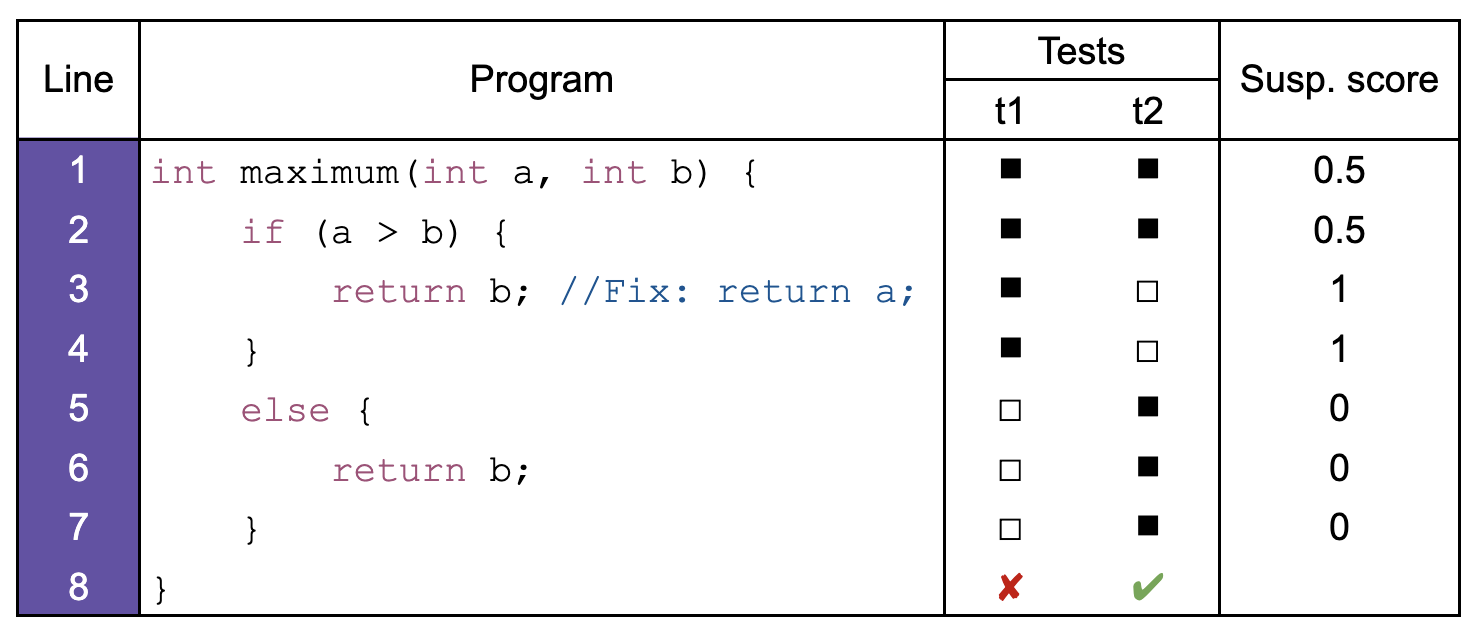
\includegraphics[width=0.8\textwidth]{figures/core/sbflExample.png}
\caption{SBFL example}
\label{fig:sbfl}
\end{figure}

Spectrum-based fault localization is a technique that aims at identifying the locations of faults in a software program by analyzing the coverage-based spectrum by running the passing and failing tests. SBFL formulas are used to compute a suspiciousness score for each program component. Usually, a score of 1 is given to the most suspicious component (usually a program statement) and a score of 0 to the least. Figure~\ref{fig:sbfl} illustrates an example of a faulty program, the coverage information about two test cases, one failing and one passing, and the suspiciousness score derived from an SBFL formula. The bug lies on line 3 in the return statement. Test case \textsc{t1} failed after covering the first 4 lines. Test case \textsc{t2} passed without having covered lines 3 and 4. We see that most suspicious lines are actually lines 3 and 4.


\subsection{Formulas}

Several formulas have been introduced in the literature. The most common ones are Tarantula~\cite{tarantula}, Ochiai~\cite{Abreu:2006yf}, DStar~\cite{wong-dstar} and Barinel~\cite{abreu2009spectrum}.

    \[
    Tarantula: \textbf{S(s)} = \frac{failed(s) / totalFailed}{failed(s) / totalFailed + passed(s) / totalPassed}
    \]
    \[
    Ochiai: \textbf{S(s)} = \frac{failed(s)}{\sqrt{totalFailed * (failed(s) + passed(s)}}
    \]
    \[
    DStar: \textbf{S(s)} = \frac{failed(s)^*}{passed(s) + (totalFailed - failed(s))}
    \]
    \[
    Barinel: \textbf{S(s)} = 1 - \frac{passed(s)}{passed(s) + failed(s)}
    \]

Where \textit{s} denotes a statement in a program, \textit{S(s)} represents the suspicious score computed for a given statement \textit{s}, \textit{passed(s)} and \textit{failed(s)} are the number of, respectively, passed and fail executions for which the statement \textit{s} was covered, and \textit{totalFailed} and \textit{totalPassed} are the total number of passing and failing executions.